\documentclass[11pt, a4paper]{article}
\usepackage{CJKutf8}
\usepackage{amsthm}
\usepackage{ulem}
\usepackage{xcolor}
\usepackage{amsmath}
\usepackage{amssymb}
\usepackage{courier}
\usepackage{geometry}
\usepackage{enumitem}
\usepackage{graphicx}
\usepackage{listings}
\usepackage{algorithm}
\usepackage{algorithmic}
\usepackage{indentfirst}
%\usepackage{float}
\usepackage[perpage,stable]{footmisc} 
\geometry{left=2.7cm, right=2.7cm, top=3cm, bottom=3cm}


\usepackage{graphics}

\usepackage[colorlinks,linkcolor=black,anchorcolor=blue,citecolor=green,
  %	CJKbookmarks=true,
]{hyperref}
\hypersetup{unicode}

\linespread{1.4}
\usepackage{indentfirst}
\setlength{\parindent}{2em}
\hypersetup{hidelinks}

\usepackage{listings}
\lstset{
  numbers=left,
  texcl=true,
  escapechar=`,
  backgroundcolor=\color{lightgray!40!white}, 
  commentstyle=\rm\color{green!30!black},
  basicstyle=\footnotesize\tt,        % the size of the fonts that are used for the code
  breakatwhitespace=false,         % sets if automatic breaks should only happen at whitespace
  breaklines=true,                 % sets automatic line breaking
  captionpos=b,                    % sets the caption-position to bottom
  extendedchars=false,              % lets you use non-ASCII characters; for 8-bits encodings only, does not work with UTF-8
  frame=single,                    % adds a frame around the code
  language=Java,                 % the language of the code
  keywordstyle=\color{blue!70}\bfseries,
  showspaces=false,                % show spaces everywhere adding particular underscores; it overrides 'showstringspaces'
  showstringspaces=false,          % underline spaces within strings only
  showtabs=false,                  % show tabs within strings adding particular underscores
  tabsize=2                       % sets default tabsize to 2 spaces
}

\begin{document}
\begin{CJK*}{UTF8}{gbsn}
  \title{\bf Java程序“字数统计器”设计报告}
  \author{马玉坤-1150310618}
  \date{2016年7月23日}
  \maketitle

  \renewcommand{\contentsname}{\textbf{目录}}
  \tableofcontents
  \newpage
  \newpage
  
  \section{题目描述}
  
  编写应用程序,统计一个文本域输入文本的行数、单词数和字符数。可在图形界面中安排一个按钮、一个文本域和一个标签,点击按钮开始统计,在标签中显示结果。
  
  \section{总体设计思想}

  向窗体添加一个标签(用来显示统计信息),一个按钮(用来执行统计),一个文本域(用来供用户输入文本)。

  标签和按钮在窗口上方,文本域在下方,用户输入一段文字后,点击“统计字数”按钮,用来显示统计信息的标签立刻显示出统计结果,分别对行数、单词数、字符数进行统计。

  \begin{center}
    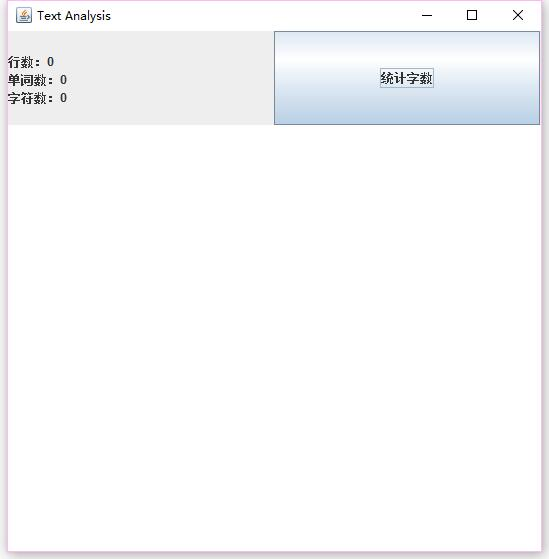
\includegraphics[height=5in]{window.jpg}
  \end{center}

  
  \section{详细设计}

  \subsection{底层容器设计}
  对于底层frame,将其布局管理器设为GridBagLayout,分为上下两行。上一行放一中间容器(lbl\_btn\_back),高度固定为40px,宽度与窗口宽度相同。下一行放一文本域(text)占满窗口剩余空间。

  \begin{lstlisting}
    // 将frame的布局管理器设为GridBagLayout,两行一列
    Container pane = frame.getContentPane();
    pane.setLayout(new GridBagLayout());

    GridBagConstraints c = new GridBagConstraints();
    // 对于上下两个格子,x方向的空白区域全部填充
    c.weightx = 1.0;  
    // 对于每个格子内部,组件把格子空间全部占满
    c.fill = GridBagConstraints.BOTH;
    c.ipady = 40;

    // 设置中间容器lbl\_btn\_back,其上放置label和button
    Panel lbl_btn_back = new Panel();
    lbl_btn_back.setLayout(new GridLayout(1, 2));
    c.gridx = 0;
    c.gridy = 0;
    c.gridwidth = 1;
    c.gridheight = 1;
    pane.add(lbl_btn_back, c);

    // 设置供用户输入的文本域
    JTextArea text = new JTextArea();
    c.gridx = 0;
    c.gridy = 1;
    c.weightx = 1.0;
    c.weighty = 1.0;
    c.gridwidth = 2;
    pane.add(text, c);
  \end{lstlisting}

  \subsection{中间容器设计}
  
  在中间容器(lbl\_btn\_back)上,使用布局管理器GridLayout分为一行两列。两个格子大小相同,分别放置标签(label)和按钮(button)。

  \begin{lstlisting}
    // 设置标签的初始内容,并加入lbl\_btn\_back上
    JLabel label
    = new JLabel("`<html>行数:0<br>单词数:0<br>字符数:0</html>`");
    lbl_btn_back.add(label);

    // 设置按钮的初始内容,并加入lbl\_btn\_back上
    JButton button = new JButton("`统计字数`");
    lbl_btn_back.add(button);
  \end{lstlisting}

  \subsection{事件监听}
  
  向button添加事件监听器监听actionPerformed事件。当按钮被点击时,更新标签内容。其中行数的统计使用text.getLineCount(),字符数的统计使用text.getText().length(),单词数的统计使用自定义方法int getWordCount(String s)。
  
  \begin{lstlisting}
    // 绑定按钮事件,当用户点击按钮时更新label内容
    button.addActionListener(
    new ActionListener() {
      public void actionPerformed(ActionEvent e) {
        label.setText("`<html>行数:`" + text.getLineCount()
        + "`<br>单词数:`" + getWordCount(text.getText())
        + "`<br>字符数:`" + text.getText().length() + "</html>");
      }
    });
  \end{lstlisting}

  \subsection{单词数目统计方法}

  在自定义的单词数目统计方法中,传入字符串s,返回s中被非英文字母隔开的连续英文字母的块数,也即满足$s[i]$为字母$\land$($i=0 \lor s[i-1]$不为字母)的$i$的个数。例如字符串$s=''abc$你$def$好$ghi''$,单词统计数目为3。

  \begin{lstlisting}
    public static int getWordCount(String s) {
    int ret = 0;
    for (int i = 0; i < s.length(); i++) {
      char ch = s.charAt(i);
      if ((ch >= 'a' && ch <= 'z') || (ch >= 'A' && ch <= 'Z')) {
        if (i == 0) {
          ret++;
        } else {
          char prev_ch = s.charAt(i - 1);
          if ((prev_ch < 'a' || prev_ch > 'z')
              && (prev_ch < 'A' || prev_ch > 'Z'))
            ret++;
        }
      }
    }
    return ret;
  }
  \end{lstlisting}
  
  \section{具体实现}

  \begin{lstlisting}

    import javax.swing.*;
    import java.awt.*;
    import javax.swing.JButton;
    import javax.swing.JFrame;
    import java.awt.event.*;
    
    public static int getWordCount(String s) {
      int ret = 0;
      for (int i = 0; i < s.length(); i++) {
        char ch = s.charAt(i);
        if ((ch >= 'a' && ch <= 'z') || (ch >= 'A' && ch <= 'Z')) {
          if (i == 0) {
            ret++;
          } else {
            char prev_ch = s.charAt(i - 1);
            if ((prev_ch < 'a' || prev_ch > 'z')
            && (prev_ch < 'A' || prev_ch > 'Z'))
            ret++;
          }
        }
      }
      return ret;
    }

      public static void main(String[] args) {
        // 设置frame标题,默认大小
        JFrame frame = new JFrame("Text Analysis");
        frame.setSize(300, 400);
        frame.setDefaultCloseOperation(JFrame.EXIT_ON_CLOSE);

        // 将frame的布局管理器设为GridBagLayout,两行一列
        Container pane = frame.getContentPane();
        pane.setLayout(new GridBagLayout());

        GridBagConstraints c = new GridBagConstraints();
        // 对于上下两个格子,x方向的空白区域全部填充
        c.weightx = 1.0;
        // 对于每个格子内部,组件把格子空间全部占满
        c.fill = GridBagConstraints.BOTH; 
        c.ipady = 40;

        // 设置中间容器lbl\_btn\_back,其上放置label和button
        Panel lbl_btn_back = new Panel();
        lbl_btn_back.setLayout(new GridLayout(1, 2));
        c.gridx = 0;
        c.gridy = 0;
        c.gridwidth = 1;
        c.gridheight = 1;
        pane.add(lbl_btn_back, c);

        // 设置供用户输入的文本域
        JTextArea text = new JTextArea();
        c.gridx = 0;
        c.gridy = 1;
        c.weightx = 1.0;
        c.weighty = 1.0;
        c.gridwidth = 2;
        pane.add(text, c);
        
        // 设置标签的初始内容,并加入lbl\_btn\_back上
        JLabel label
        = new JLabel("`<html>行数:0<br>单词数:0<br>字符数:0</html>`");
        lbl_btn_back.add(label);

        // 设置按钮的初始内容,并加入lbl\_btn\_back上
        JButton button = new JButton("`统计字数`");
        lbl_btn_back.add(button);

        // 绑定按钮事件,当用户点击按钮时更新label内容
        button.addActionListener(
        new ActionListener() {
          public void actionPerformed(ActionEvent e) {
            label.setText("`<html>行数:`" + text.getLineCount() +
            "`<br>单词数:`" + getWordCount(text.getText()) +
            "`<br>字符数:`" + text.getText().length() + "</html>");
          }
        });

        // 显示窗体
        frame.setVisible(true);
      }
    }

  \end{lstlisting}

  \section{运行结果}
  \begin{center}
    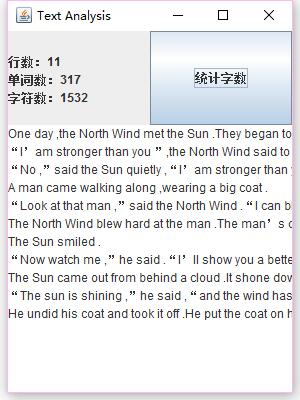
\includegraphics[height=5in]{result.jpg}
  \end{center}
  
  \newpage

\end{CJK*}
\end{document}
